\documentclass[10pt, a4paper,openany]{book}
\usepackage{graphicx} % Required for inserting images
\usepackage{needspace}
\usepackage{tikz}
\usetikzlibrary{positioning}
\renewcommand{\figurename}{Figura}

\DeclareUnicodeCharacter{0301}{\'{e}}
\usepackage[
backend=biber,
style=numeric,
sorting=none
]{biblatex}
\addbibresource{Citas.bib}


\usepackage{amsthm}

\theoremstyle{definition}
\newtheorem{exmp}{Ejemplo}[section]


\title{Ontología}
\author{Kelvin José Ojeda Quiroz}
\date{Mayo 2023}

\begin{document}

\maketitle

\section{Marco teórico}
\label{S: Marco teórico}
\subsection{Antecedentes}
\label{SS: Antecedentes}
La vasta cantidad de recursos en la web, que carecen de una estructura y definición adecuadas, se convierte en un problema evidente para cualquier usuario de Internet.
Esta abrumadora cantidad de recursos conlleva el inconveniente de tener que contar con lo que hoy conocemos como ``información irrelevante" dentro de la web \cite{bonilla_web_2006}.

En el contexto actual de 2023, una posible causa subyacente de esta situación en la infraestructura web es el uso predominante del lenguaje de programación HTML.
Aunque HTML permite la inclusión de hipertexto, imágenes, sonido y multimedia, se considera principalmente un lenguaje estructural de maquetación \cite{bonilla_web_2006}.
Sin embargo, a pesar de su capacidad para describir la estructura y el formato de los contenidos web, HTML carece de una representación semántica clara de los datos.
Se centra en la presentación visual y la estructura superficial del contenido, sin proporcionar mecanismos para definir relaciones y significados más profundos entre los elementos.
Esta limitación conlleva a una falta de estructura y definición adecuadas en la web, lo cual puede resultar en una gran cantidad de recursos poco estructurados e información irrelevante.

En 1999, Tim Berners-Lee, conocido como el padre de la WWW (World Wide Web), junto con James Hendler y Ora Lassila, presentaron por primera vez una serie de requisitos hipotéticos sobre los cuales se debería basar la futura Web Semántica.
Este discurso generó numerosas discusiones académicas en aquel momento, sentando las bases para la materialización de muchas de las ideas propuestas.
Desde entonces, se ha ido formando un consenso en torno a la idea de que el futuro de la web se encuentra en la investigación en inteligencia artificial de naturaleza cualitativa similar a la humana \cite{noauthor_scientific_nodate}.

Así, los primeros conceptos relacionados con la ontología comienzan a formularse, ya que los primeros pasos de la Web Semántica se basan en la adopción generalizada de XML, presente desde los inicios en la creación de páginas web, como HTML.
Sin embargo, HTML se enriquece con propiedades de metadatos que permiten una descripción explícita y ontológica del contenido de la información incrustada en las páginas web que se desean describir \cite{bonilla_web_2006}.
Esta inclusión de metadatos en HTML proporciona un marco adicional para expresar de manera más precisa y formal las relaciones y significados de los datos, facilitando así el análisis y la interpretación de la información en un contexto semántico más profundo.
Al enriquecer HTML con metadatos, se mejora su capacidad para representar y organizar la información de manera más notoria tanto para los usuarios como para las máquinas, impulsando así la evolución hacia una web más estructurada y con mayor significado.
De esta manera, surge la necesidad de explicitar los escenarios en los cuales se requiere el desarrollo de una ontología, como se muestra a continuación \cite{filho_ontology_nodate}:
\begin{itemize}
    \item \textbf{Compartir el entendimiento común de la estructura de la información entre personas o agentes de software}
    
    Esto implica que tanto las personas como los programas informáticos tienen una comprensión clara y compartida de cómo está organizada la información.
    Esta compartición de conocimiento puede mejorar la eficiencia en la comunicación y la gestión de la información.
    Además, cuando los programas informáticos comparten esta comprensión de la estructura de la información, se logra una mejora en la precisión y eficiencia en el procesamiento y gestión de la información.
    Por ejemplo, si varios sitios web médicos comparten y publican la misma ontología subyacente de términos que utilizan, los agentes de software pueden extraer y agregar información de estos sitios diferentes.
    Esta información agregada puede ser utilizada para responder solicitudes de usuarios o como datos de entrada para otras aplicaciones.
    \item \textbf{Permitir la reutilización de conocimiento de un dominio}

    La utilización de una ontología clara y descriptiva en un dominio específico permite su reutilización en diferentes proyectos o aplicaciones relacionadas con dicho dominio.
    Si un grupo de investigadores ha desarrollado una ontología detallada, otros pueden simplemente aprovecharla y reutilizarla en sus propios dominios.
    Esto evita tener que empezar desde cero en cada proyecto y facilita el intercambio de conocimiento y recursos entre diferentes equipos de investigación.
    Al utilizar una ontología existente, se ahorra tiempo y esfuerzo en la creación de nuevas estructuras y se fomenta la colaboración y la construcción sobre el trabajo de otros.

    \item \textbf{Hacer explicitas suposiciones de un dominio}
    
    Brinda la capacidad de ajustar o cambiar estas suposiciones a medida que nuestro conocimiento o comprensión del dominio evoluciona con el tiempo.
    Es especialmente relevante en áreas de conocimiento que experimentan cambios frecuentes o están sujetas a avances tecnológicos y nuevas comprensiones del dominio.
    Al hacer estas suposiciones explícitas y flexibles, se aumenta la capacidad de adaptación y flexibilidad del proyecto o implementación, permitiendo ajustes según las condiciones cambiantes o la evolución de la comprensión del dominio.
    \needspace{2\baselineskip}
    
    \item \textbf{Analizar el conocimiento de un dominio}
    
    Al tener una especificación clara y declarativa de los términos que se utilizan en un dominio específico a través de una ontología, se puede analizar y comprender de manera más efectiva el conocimiento relacionado con ese dominio.
    Esto es especialmente útil cuando se desea reutilizar ontologías existentes o ampliarlas para cubrir nuevas áreas dentro del mismo dominio.
    Al tener una definición formal y precisa de los términos, es posible aplicar herramientas y técnicas de análisis formales para entender cómo se relacionan los diferentes términos, cómo se pueden agrupar en clases o categorías y cómo se pueden aplicar diferentes reglas y restricciones a los términos en diferentes situaciones.

     
\end{itemize}
\subsection{Definición de ontología}
\label{SS: Definición de ontología}
Inicialmente, el concepto de ontología ha sido interpretado por diversos actores, siendo uno de los más destacados Gruber \cite{gruber_toward_1995}, quien proporciona una definición aproximada al referirse a la ontología como ``una especificación explícita y formal de una conceptualización".
En términos más simples, podemos entender una ontología como un conocimiento común y compartido acerca de un dominio, que puede ser comunicado tanto por humanos como por sistemas computacionales, utilizando conceptos asociados específicamente para la Web Semántica.
Sin embargo, desde una perspectiva técnica, el término ontología adquiere un significado complementario al propuesto por Gruber.
Estos conceptos son representados como clases o conceptos, y se definen propiedades para cada uno de ellos, describiendo características y atributos, como roles o propiedades, así como restricciones sobre dichos roles \cite{filho_ontology_nodate}.
\subsection{Elementos de una ontología}
\label{SS: Elementos de una ontología}
En base a las definiciones de la subsección \ref{SS: Definición de ontología}  se puede identificar los componentes fundamentales que conforman una ontología, los cuales se detallan a continuación \cite{filho_ontology_nodate}.
\begin{itemize}
    \item \textbf{Clases: }Son elementos centrales en una ontología, ya que representan conceptos dentro de un dominio.
    \item \textbf{Subclases: }Son representaciones más específicas de conceptos que se encuentran dentro de una superclase más general.
    \item \textbf{Slots: }Son utilizados para describir las propiedades de las clases y las instancias.
\end{itemize}


\label{Ej: Ontologia marco teorico}

Con el objetivo de comprender mejor los conceptos asociados a una ontología y a sus elementos, a continuación, se proporciona un ejemplo, adaptado de \cite{filho_ontology_nodate}, que ilustra las diferentes partes que conforman una ontología: 
\begin{exmp}
% Corregir los terminos de ejemplos dentro de la etiqueta ejemplo
Consideremos la clase ``Vino", la cual representa a todos los tipos de vinos. 
Los vinos específicos serían considerados como instancias de esta clase. 
%Además, es importante destacar que una clase puede tener subclases que representan especializaciones de la superclase. 
Podemos dividir la clase``Vino" en subclases como ``Vino Tinto", ``Vino Blanco" y ``Vino Rosado". 
Otro aspecto relevante son los ``Slots", consideremos la instancia de vino llamada ``Chateau Lafite Rothschild Pauillac".
Esta instancia pertenece a la clase ``Vino" y se caracteriza por ser producida en la bodega ``Chateau Lafite Rothschild".
En este caso, los ``Slots" o propiedades del vino podrían describir su sabor, cuerpo, nivel de azúcar y otros atributos como el productor de dicho vino.
Cada instancia de la clase ``Vino" y su subclase ``Vino Pauillac" tiene un atributo denominado ``productor", el cual es una instancia de la clase ``Establecimiento vinícola", tal como se ilustra en la Figura~\ref{fig:Ejemplo_ontologia_marco_teorico}.
Por otro lado, todas las instancias de la clase "Establecimiento vinícola" poseen un atributo llamado ``produce", el cual se refiere a todos los vinos pertenecientes a la clase ``Vino" y sus subclases. Este atributo representa que los vinos son producidos por dicho establecimiento vinícola.
\end{exmp}
    



\begin{figure}
    \centering
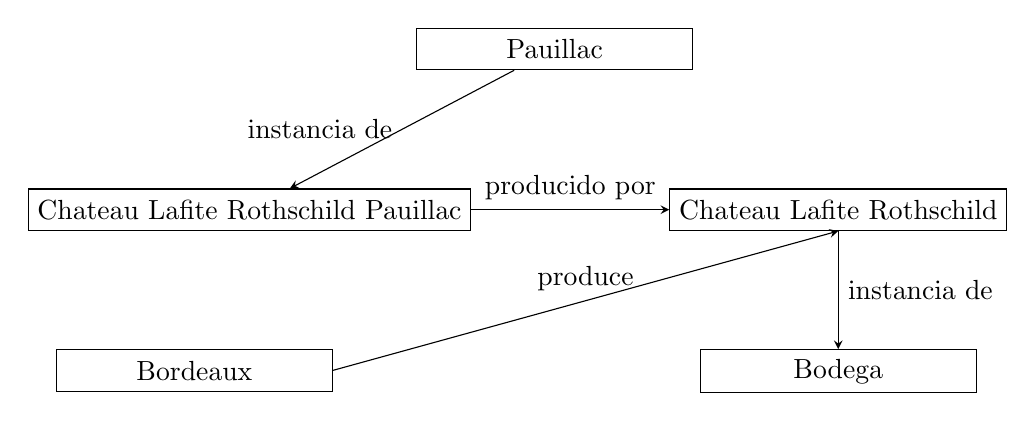
\begin{tikzpicture}[
  class/.style={rectangle, draw, text centered, minimum height=1.5em, minimum width=3.5cm},
  relation/.style={->, >=stealth}
]

% Clases
\node[class] (pauillac) {Pauillac};
\node[class, below left=1.5cm and -0.7cm of pauillac] (chateaulafite) {Chateau Lafite Rothschild Pauillac};
\node[class, below right=1.5cm and -0.3cm of pauillac] (chateaubodega) {Chateau Lafite Rothschild};
\node[class, below=1.5cm of chateaubodega] (bodega) {Bodega};
\node[class, below=1.5cm of chateaulafite, xshift=-0.7cm] (bordeaux) {Bordeaux};

% Relaciones
\draw[relation] (pauillac) -- (chateaulafite) node[midway, left] {instancia de};
\draw[relation] (chateaubodega) -- (bodega) node[midway, right] {instancia de};
\draw[relation] (chateaulafite) -- (chateaubodega) node[midway, above] {producido por};
\draw[relation] (bordeaux.east) -- (chateaubodega.south) node[midway, above] {produce};

\end{tikzpicture}
    \caption{Ontología en el dominio de vinos.}
    %Los enlaces directos representan los slots, es decir, las propiedades de las clases. Por otro lado, los enlaces internos representan las instancias o subclases de una clase}
    \label{fig:Ejemplo_ontologia_marco_teorico}
\end{figure}



%\bibliographystyle{unsrt}
%\bibliography{Citas}
\printbibliography[title={Referencias}]

\end{document}
